\section{Transformator}
		
	\subsection{Trafomodelle}
%		\subsubsection{Grundstrucktur des Trafo}
%			\begin{tabular}{p{7cm}p{4.5cm}p{5cm}}
%	        	\textbf{} &
%	        		\begin{minipage}{4.5cm}
%		            	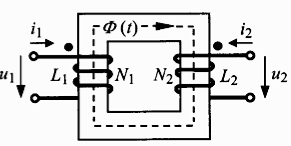
\includegraphics[width=3.5cm]{bilder/GrundstruckturTrafo.png}
%		            \end{minipage} \\
%	        \end{tabular}
		\subsubsection{Der ideale Trafo}
			\begin{tabular}{p{7cm}p{4.5cm}p{5cm}}
				Übersetzungsverh\"altnis &
					$\text{ü} = \frac{|\underline{U}_1|}{|\underline{U}_2|} =
					\frac{|\underline{I}_2|}{|\underline{I}_1|} = \frac{N_1}{N_2}$ &
					\begin{minipage}{4.5cm}
						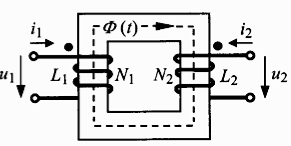
\includegraphics[width=3.5cm]{bilder/GrundstruckturTrafo.png}
					\end{minipage} \\
				Leistungsbilanz &
					$\underline{S}_1 = \underline{S}_2$ 
					oder $\underline{U}_2 \cdot \underline{I}_2^* = \underline{U}_1 \cdot \underline{I}_1^*$ \\
				Scheinwiderstandsübersetzung &
					$\underline{Z}_{aU} = \frac{|\underline{U}_1|^2}{|\underline{U}_2|^2} \cdot \underline{Z}_a = \text{ü}^2 \cdot \underline{Z}_a$ &
					\begin{minipage}{4.5cm}
	            		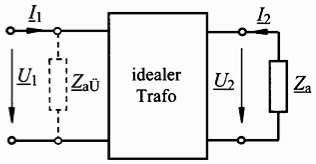
\includegraphics[width=3.5cm]{bilder/IdealerTravoImpedanzwandler.png}
	            	\end{minipage}
			\end{tabular}

		
		\subsubsection{Verlustloser und Streuungsfreier Trafo (VST)}
			\renewcommand{\arraystretch}{1.5}
\textbf{Induktionsgesetz}\\
		\begin{tabular}[c]{p{8.7cm}}
			$u_i= \mp \dot{\Phi} = \mp \frac{d}{dt} \int \vec{B} \cdot
			\vec{dA}\qquad $ \parbox{3cm}{\tiny{$- \Rightarrow B,u_i $
			Rechtsschraube\\ $+ \Rightarrow B,u_i $
			Linksschraube}}
			\\
			
			$u_i= \mp \dot{\Psi}\qquad$ , meist $\; u_i = \mp
			N\cdot\dot{\Phi}$		
		\end{tabular}
		\parbox{8cm}{Durchsetzt das sich \"andernde Magnetfeld einer stromdurchflossenen Spule
					eine zweite Spule, so wird auch in dieser eine Spannung
					(=Gegeninduktionsspannung) induziert.}	

\begin{multicols}{2}
 		\textbf{Gegeninduktion} ($M_{\textcolor{red}{X}\textcolor{green}{Y}}; \textcolor{red}{X}$: Wirkung,
 		$\textcolor{green}{Y}$: Ursache)\\
		\begin{tabular}{ll}
  		Gegeninduktivit\"at
  			& $M_{21} = \frac{\Psi_{m21}}{i_1}$ Meist $= \frac{N_2 \phi_{m21}}{i_1}$\\ 
  			(wenn $\mu$ = const.) & $M = k \cdot \sqrt{L_1 L_2} = M_{21} = M_{12} $  \\
  			Gegeninduktionsspannung
  			& $u_{21} = \dot{\Psi}_{21} = M_{21} \frac{di_1}{dt}$ \\
		\end{tabular}\\

  		\textbf{Transformatorgleichungen}\\
		$\boxed{u_1 = L_1 \dfrac{di_1}{dt} \textcolor{red}{+}\textcolor{green}{-}M_{12}
		\dfrac{di_2}{dt} = L_1 \dfrac{di_1}{dt} \textcolor{red}{-}\textcolor{green}{+}M_{12} \dfrac{di_b}{dt}}$ \\
		$\boxed{u_2 = L_2 \dfrac{di_2}{dt}\textcolor{red}{+}\textcolor{green}{-} M_{21}
		\dfrac{d i_1}{dt} = -L_2 \dfrac{di_b}{dt}
		\textcolor{red}{+}\textcolor{green}{-} M_{21} \dfrac{d i_1}{dt}}$\\
		Im Bildbereich:\\
		$\underline{U}_1 = j\omega\cdot L_1 \cdot \underline{I}_1 + j\omega\cdot M \cdot \underline{I}_2$\\
		$\underline{U}_2 = j\omega\cdot L_2 \cdot \underline{I}_2 + j\omega\cdot M \cdot \underline{I}_1$\\
  			
	  	\textbf{Idealer Trafo}\\ 
	  	$"u = \dfrac{u_1}{u_2} = \dfrac{N_1}{N_2} = \sqrt{\dfrac{L_1}{L_2}}$ $\qquad$ (im Leerlauf:
	  	$\dfrac{1}{"u} = k \sqrt{\dfrac{L_2}{L_1}}$)\\

  		\textbf{Verlustbehafteter Trafo}
  		\begin{list}{$\bullet$}{\setlength{\itemsep}{0cm} \setlength{\parsep}{0cm} \setlength{\topsep}{0cm}} 
          \item Prim\"arstrom im Leerlauf: $L_H$
          	(ideal $L_H \rightarrow \infty)$
          \item Hysterese- \& Wirbelstromverluste: $R_{Fe}$ \newline
          	(ideal: $R_{Fe}\rightarrow \infty$) 
          \item Kupferwiderst\"ande: $R_{Cu1}, R_{Cu2}$
          	(ideal: $R_{Cu}
          \rightarrow 0$)
          \item Streufluss (Kopplung): $L_{\sigma1}, L_{\sigma2}$
          	(ideal: $L_{\sigma} \rightarrow 0$)
        \end{list}

	\columnbreak
  		\begin{flushleft}
  		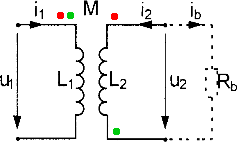
\includegraphics[width=4cm]{bilder/trafo-kopplung.png} \\
  		\small{\textcolor{red}{Gleichsinnig} / \textcolor{green}{Gegensinnig}} \\
  		\vspace{1cm}

	  	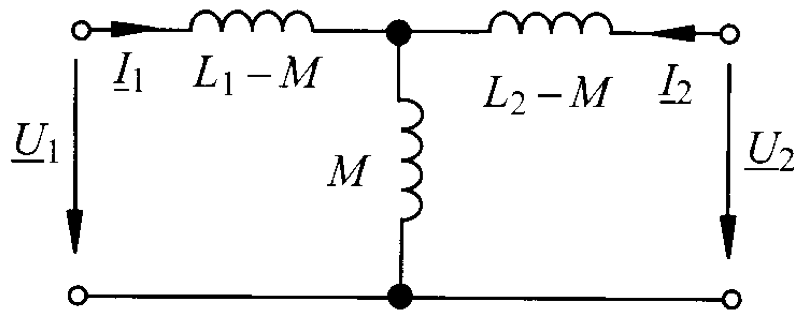
\includegraphics[width=5cm]{bilder/T_Ersatzschaltbild_VST.png}\\
		\end{flushleft}  	
	
\end{multicols}
\renewcommand{\arraystretch}{1} 
		\renewcommand{\arraystretch}{1.5}	
		\subsubsection{Transformatoren-Hauptgleichung (gilt bei Leerlauf)}
			\begin{tabular}{p{7cm}p{4cm}p{6cm}}
      			$\boxed{U_{10} = \frac{2\pi}{\sqrt{2}}N_1 \cdot f \cdot \hat{B}_1 \cdot A}$
      			& 	$|\hat{u}_{10}| = \hat{i}_0 \cdot \omega \cdot L_1$ & Mit $\omega = 2\pi \cdot f$ und $L_1 = N_1 \cdot \frac{\hat{\Phi}_{10}}{\hat{i}_0}$ folgt: \\
      		
				$\boxed{U_{20} = \frac{2\pi}{\sqrt{2}}N_2 \cdot f \cdot \hat{B}_1 \cdot A}$
				& $|\hat{u}_{10}| = 2\pi N_1 \cdot f \cdot \hat{\Phi}_{10} $
            	& Leerlauferregerfluss durchsetzt magn. Kreis $\bot$:$ \hat{\Phi}_{10} = \hat{B}_1 \cdot A $. So folgt: \\
				
				wobei $\frac{2\pi}{\sqrt{2}} = 4.44$ und $\hat{B} \cdot A = \hat{\Phi}$ &
				$|\hat{u}_{10}| = 2\pi N_1 \cdot f \cdot \hat{B}_1 \cdot A	$
			\end{tabular}
		\renewcommand{\arraystretch}{1}	
		
	\newpage
	\subsection{Der reale (einphasige) Transformator}
		Für dreiphasige Trafos müssen die angegebenen Werte zuerst normiert werden (siehe Kapitel 3).
	
		\renewcommand{\arraystretch}{1.25}
		\subsubsection{Ersetzen der magnetischen Kopplung}
			\begin{tabular}{p{5.8cm}p{7.3cm}p{4.5cm}}
            	Spannung, Strom &
            		$U_2' = U_2 \cdot \frac{N_1}{N_2}$ \quad 
            		$I_2' = I_2 \cdot \frac{N_2}{N_1}$ \\
            	Nennstrom & 
            		$I_N = S_N / U_N$ \\
            	Widerstand, &
            		$R_2' = R_2 \cdot (\frac{N_1}{N_2})^2$\quad $ Z_2' = Z_2\cdot (\frac{N_1}{N_2})^2$\\
            	Streufluss&
            		$X_{\sigma 2}' = X_{\sigma 2} \cdot (\frac{N_1}{N_2})^2$ \\
            	Vollst\"andiges Ersatzschaltbild &
            	\begin{minipage}{7cm}
            		\adjustbox{width=7cm}{\begin{circuitikz}[european]
	\draw (0,0) coordinate (In1) {} 
		to[short, *-, i=$\underline{I_1}$] ++(1,0)
		to[R, l=$R_1$] ++(2,0)
		to[L, l=$jX_{\sigma 1}$] ++(2,0)
		to[short, -*] ++(1,0) coordinate (middle1) {}
		to[short] ++(1,0)
		to[L, l=$jX'_{\sigma 2}$] ++(2,0)
		to[R, l=$R'_2$] ++(2,0)
		to[short, -* ,i<=$\underline{I_2}$] ++(1,0) coordinate(Out1);
	\draw (middle1) to[short, -*] ++(0,-1) coordinate (middle2) {};
	\draw (middle2) -- ++(-1,0) 
		to[R, l=$R_{Fe}$] ++(0,-2)
		to[short, -*] ++(1,0) coordinate(middle3)
		to[short, -*] ++(0,-1) coordinate(middle4);
	\draw (middle2) -- ++(1,0)
		to[L, l=$jX_h$] ++(0,-2)
		to[short] (middle3);
	\draw (middle4) to[short, -*] ++(-6,0) coordinate(In2);
	\draw (middle4) to[short, -*] ++(6,0) coordinate(Out2);
	\begin{scope}[
		shorten <=10pt,
		shorten >= 10pt,
		->
	]
		\draw (In1) -- (In2) node[midway, right] {$\underline{U_1}$};
		\draw (Out1) -- (Out2) node[midway, left] {$\underline{U'_2}$};
	\end{scope}
\end{circuitikz}}
            	\end{minipage}
            	&
					\begin{minipage}{4.5cm}
                    	\tiny
                    		$R_1, R_2'$: Widerstand Spule\\ \\
                    		$jX_{\sigma 1}, jX_{\sigma 2}'$: Streufluss Spule\\ \\
                    		$R_{Fe}$: Eisenverlust\\ \\
                    		$jX_h$: Hauptfluss Spule\\
                    \end{minipage} \\ \\
				Systemgleichung des realen Trafo &
					$\underline{U}_1 = R_1\cdot\underline{I}_1 + jX_{\sigma 1}\cdot\underline{I}_1 + jX_h\cdot(\underline{I}_1+\underline{I}_2')$ \\
					&$\underline{U}_1 = R_1\cdot\underline{I}_1 + j\omega L_{\sigma 1}\cdot\underline{I}_1 + j\omega L_m\cdot(\underline{I}_1+\underline{I}_2')$ \\
					& $\underline{U}_2' = R_2'\cdot\underline{I}_2' + jX_{\sigma 2}'\cdot\underline{I}_2' + jX_h\cdot(\underline{I}_1+\underline{I}_2')$

            \end{tabular}
            
            	Für mittlere Transformatorenleistungen erbgeben sich etwa folgende Relationen zwischen
            	den einzelnen $R$s und $X$s:
            	$$\boxed{ R_1 : R_2' : X_{\sigma 1} : X_{\sigma 2}' : X_h : R_{Fe} \approx 1:1:2:2:1000:10000}	$$
    
        \renewcommand{\arraystretch}{1.5}   
		\subsubsection{Leerlauf und Magnetisierung}
			\begin{tabular}{p{5cm}p{6cm}p{7cm}}
            	Rechnen &
            		\begin{minipage}{13cm}
                    	Mit Leerlaufdaten $R_{Fe}$ und $X_h$ ausrechnen. \underline{$R_1$ und $X_{\sigma1}$ vernachl\"assigen.}
                    \end{minipage} \\ \\
            	Induktiver Leerlaufstrom &
            		$\underline{I}_{10} = \underline{I}_{1Fe} + \underline{I}_{1\mu}$ \quad $(\underline{I}_{1\mu} \gg \underline{I}_{1Fe})$ &
            		\begin{minipage}{7cm}
	            		\adjustbox{width=6cm}{\begin{circuitikz}[european]
	\draw (0,0) coordinate (In1) {} 
		to[short, *-, i=$\underline{I}_{10}$] ++(1,0)
		to[R, l=$R_1$] ++(2,0)
		to[L, l=$jX_{\sigma 1}$] ++(2,0)
		to[short, -*] ++(1,0) coordinate (middle1) {}
		to[short, -* ,i<=\mbox{$\underline{I}_2 = 0$}] ++(3,0) coordinate(Out1);
	\draw (middle1) to[short, -*] ++(0,-1) coordinate (middle2) {};
	\draw (middle2) 
		to[short, i_=$\underline{I}_{1Fe}$] ++(-1,0) 
		to[R, l=$R_{Fe}$] ++(0,-2)
		to[short, -*] ++(1,0) coordinate(middle3)
		to[short, -*] ++(0,-1) coordinate(middle4);
	\draw (middle2) 
		to[short, i=$\underline{I}_{1\mu}$] ++(1,0)
		to[L, l=$jX_h$] ++(0,-2)
		to[short] (middle3);
	\draw (middle4) to[short, -*] ++(-6,0) coordinate(In2);
	\draw (middle4) to[short, -*] ++(3,0) coordinate(Out2);
	\begin{scope}[
		shorten <=10pt,
		shorten >= 10pt,
		->
	]
		\draw (In1) -- (In2) node[midway, right] {$\underline{U}_{10}$};
		\draw (Out1) -- (Out2) node[midway, right] {$\underline{U}'_{20}$};
	\end{scope}
\end{circuitikz}}
	            	\end{minipage} \\ \\
				Magnetisierungsstrom &
					\multicolumn{2}{l}{
					$i_\mu = \sqrt{2}I_{\mu 1}\cdot \sin(\omega t) + \sqrt{2}I_{\mu 3}\cdot \sin(3\omega t) + \ldots + \sqrt{2}I_{\mu m}\cdot \sin(m\omega t)$
					\quad$(m=2n+1 \hspace{0.3cm} n\in \mathbb{N}_0)$ 
					}\\
				&
					$I_{\mu RMS} = \sqrt{{I_{\mu 1}}^2 + {I_{\mu 3}}^2 +\ldots+ {I_{\mu m}}^2} $\\ \\
				Leerlaufverluste &
					$P_0 = P_{0Cu} + P_{0Hy} + P_{0Wi}$ \\
				Kupferverluste &
					$P_{Cu} = {I_0}^2 \cdot R_{Cu}$\\
				Hystreseverluste &
					$P_{Hy} \sim f \cdot B^2$ \\
				Wirbelstromverluste &
					$P_W = c_W \cdot f^2 \cdot B^2$ &
					$c_W$ ist materialabh\"angige Konstante \\
				Relativer Leerlaufstrom &
					$i_{0N} = \frac{I_{0N}}{I_{1N}}$ &
					$I_{1N}$ ist eingangsseitiger Nennstrom \\
				Eisenverluststrom &
					$I_{Fe} \approx \frac{P_{0N}}{U_{1N}} \approx I_0 \cdot \cos(\varphi_0)$ \\
				Eisenverlustwiderstand &
					$R_{Fe} \approx \frac{U_{1N}^2}{P_{0N}} \approx \frac{P_{0N}}{I_{Fe}^2}$ \\
				Hauptreaktanz &
					$X_h = L_h \omega = \frac{U_{1N}}{I_{\mu}} = \frac{U_{1N}^2}{Q_{0N}}
					=
					\frac{Q_{0N}}{I_{\mu}^2}$
					& mit $Q_{0N} = \sqrt{S_{0N}^2 - P_{0N}^2}$ \\
				Magnetisierungsstrom &
					$I_\mu = I_{0} \cdot \sin(\varphi_0) = \sqrt{I_0^2 - I_{Fe}^2}$&
					oder $\hat{I}_{\mu} = \frac{\hat{H}_{Fe} \cdot l_{Fe}}{N_1} \Leftrightarrow I_{\mu} = \frac{\hat{H}_{Fe} \cdot l_{Fe}}{\sqrt{2}\cdot N_1}$ \\
				&$I_\mu = I_1-\frac{N_1}{N_2}\cdot I_2$\\

				Leistungsfaktor im Leerlauf &
					$\cos(\varphi_0) = \frac{P_{0N}}{I_{0N} \cdot U_{1N}}$ & \multirow{2}{*}{\adjustbox{height=2cm}{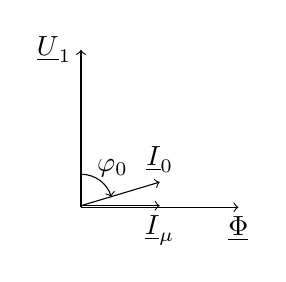
\begin{tikzpicture}
	\begin{scope}[->]
		\draw (0,0) -- +(0,2) node[left] {$\underline{U}_1$};
		\draw (0,0) -- +(2,0) node[below] {$\underline{\Phi}$};
		\draw (0,0.02) -- +(1,0) node[below] {$\underline{I}_\mu$};
		\draw (0,0.02) -- +(1,0.3) node[above] {$\underline{I}_0$};
		\draw (0,0.42) arc (90:16:0.4);
	\end{scope}
	\draw (0.4,0.5) node {$\varphi_0$};	
\end{tikzpicture}% }}\\\\
				Leerlaufstrom &
					$I_0 = \sqrt{{I_{\mu}}^2 + {I_{Fe}}^2}$
            \end{tabular}
            
        \renewcommand{\arraystretch}{1.25}
		\subsubsection{Kurzschluss}
			\begin{tabular}{p{5cm}p{6cm}p{7cm}}
				\multicolumn{3}{p{18cm}} {
					Mit Kurzschlussdaten $R_1$ und $X_{\sigma1}$ ausrechnen. \underline{$R_{Fe}$ und $X_h$ vernachl\"assigen.}
				}
			
	            \\
				Kurzschlussimpedanz &
					$\underline{Z}_k = R_k + jX_k = \frac{\underline{U}_k}{\underline{I}_k}$& \multirow{2}{*}{
										\adjustbox{width=6.5cm}{\begin{circuitikz}[european]
	\draw (0,0) node (in) {} to[short, *-, i=$\underline{I_1}$] ++(1,0)
		to[R, l=$R_1$] ++ (2,0)
		to[L, l=$jX_{\sigma 1}$] ++(2,0)
		to[L, l=$jX^`_{\sigma 2}$] ++(2,0)
		to[R, l=$R^`_2 $] ++(2,0)
		-- ++(0,-2) to[short, -*] (0,-2) node (out) {};
	\draw[shorten >= 5pt, shorten <= 5pt, ->] (in) -- (out)
		node[midway, right] {$\underline{U_1}$};	
\end{circuitikz}}
											              }\\
					& $Z_k = \frac{U_k}{I_k}$ & \\
					& $R_k = R_1 + R_2' = \cos{\varphi_k} \cdot Z_k  = \frac{P_k}{I_k^2}$  \\
					& $X_k = X_{\sigma1} + X_{\sigma2}' = \sin{\varphi_k} \cdot Z_k = \frac{Q_k}{I_k^2}$ \\
				Leistungsfaktor im Kurzschluss &
					$\cos(\varphi_k) = \frac{P_k}{U_k \cdot I_k} = \frac{P_k}{S_k}$	
					& $U_R = U_k \cos\varphi_k$\\
					& $P_k = I_k^2 \cdot R_k$ 					
					& $U_\sigma = U_k \sin\varphi_k$ \\
					& & $R_k=\frac{U_R}{I_k} \qquad X_k = \frac{U_\sigma}{I_k}$\\
				Dauer-Kurschluss-Strom&
					$ \underline{I}_{1k} = \frac{\underline{U}_1}{\underline{Z}_k}$\\
				Nennkurzschlussspannung&
					$ U_Z = I_{1N} \cdot Z_k$\\	
				&	$ u_z = \frac{U_Z}{U_{1N}}$
             \end{tabular}
		\renewcommand{\arraystretch}{1.5}
	
		\subsubsection{Spannungs\"anderung bei Belastung}
		\textbf{Komplexe Rechnung}\\
			\begin{tabular}{p{5cm}p{5cm}p{6cm}}
	            		$\boxed{\underline{U}_1 =
	            		\underline{U}_R+\underline{U}_X+\underline{U}_2'}$ & 
	            		$\boxed{\underline{I}_2' = \underline{I}_1}$ &
	            		\multirow{3}{*}{
	            		\parbox{6cm}{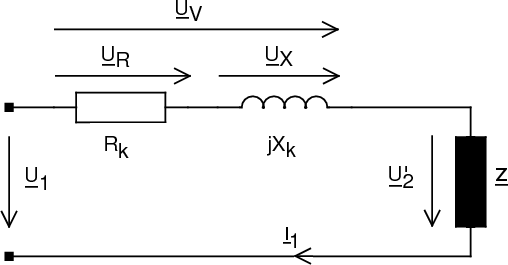
\includegraphics[width=5cm]{bilder/ErsatzschaltbildTrafoLast.png}}}
	            			            	\\		
	            		$\underline{U}_R=R_k \cdot \underline{I}_1$ &
	            		$\underline{U}_X=jX_k \cdot \underline{I}_1$ \\
	            		$\underline{U}_2'=\underline{U}_2 \cdot "u = \underline{I}_2' \cdot \underline{Z}'  $\\
	            		$\underline{Z}' = \underline{Z} \cdot {"u}^2$ \\
            \end{tabular}\\
		\renewcommand{\arraystretch}{1.0}

		\textbf{Graphische Rechnung}\\
			\begin{tabular}{p{8cm}|p{10cm}}
	 			\textbf{Zeigerdiagramme} & \textbf{Kappsches Dreieck}\\
	 			
				\begin{minipage}{8cm}
	            	\begin{multicols}{3}
	            	  \adjustbox{width=2.4cm, set vsize={7cm}{0cm}}{\begin{tikzpicture}
  \begin{scope}[->]
    \draw (0,-5) -- (0,-1) node[midway, right] {$\underline{U}_2'$};
    \draw[green!50!black] (0,-1) -- (0,0) node[midway, right] {$\underline{U}_R$};
    \draw[blue] (0,0) -- (-2,0) node[midway, above] {$\underline{U}_X$};
    \draw[violet] (0,-5) -- (-2,0) node[midway, left] {$\underline{U}_1$};
    \draw[blue!60!white] (0,-1) -- (-2,0) node[midway, below] {$\underline{U}_V$};
    \draw[red] (0.01,-5) -- (0.01,-4) node[midway, right] {$\underline{i}_1$};
   \end{scope}
   
  % Rechter Winkel
   \rechterWinkel{0,0}{180}
   % Schraffierte Fläche
   \draw[pattern=north east lines, pattern color=black!30] (0,-1) -- (0,0) -- (-2,0);   
\end{tikzpicture}}
	            	  
	            	  \columnbreak
	            	  
	            	  \adjustbox{width=2.2cm, set vsize={7cm}{0cm}}{\begin{tikzpicture}
  \begin{scope}[->]
    \draw (0,-5) -- (0,-1) node[midway, right] {$\underline{U}_2'$};
    
    \draw[green!50!black] (0,-1) -- (1,0) node[midway, right] {$\underline{U}_R$};
    \draw[blue] (1,0) -- (-1,2) node[midway, right] {$\underline{U}_X$};    
    \draw[blue!60!white] (0,-1) -- (-1,2) node[midway, right] {$\underline{U}_V$};    
    
    \draw[violet] (0,-5) -- (-1,2) node[midway, left] {$\underline{U}_1$};    
    
    \draw[red] (0,-5) -- (1,-4) node[midway, right] {$\underline{I}_1$};
   \end{scope}
   
  % Rechter Winkel
   \rechterWinkel{1,0}{133}
   % Schraffierte Fläche
   \begin{pgfonlayer}{bg}
     \fill[pattern=north east lines, pattern color=black!20] (0,-1) -- (1,0) -- (-1,2);
   \end{pgfonlayer}
   
   % Phi
   \begin{scope}[<-]
   \draw (0,-1) -- (0,-0.1);
   \draw (0,-1) +(90:0.5cm) arc[radius=0.5cm, start angle=90, delta angle=-44] node[above] {$\varphi$};
   \draw (0,-5) +(90:0.5cm) arc[radius=0.5cm, start angle=90, delta angle=-44] node[above] {$\varphi$};
   \end{scope}
   
\end{tikzpicture}}
	            	  
	            	  \columnbreak
	            	  
	            	  \adjustbox{width=2.8cm, set vsize={7cm}{0cm}}{\begin{tikzpicture}
  \begin{scope}[->]
    \draw (0,-5) -- (0,-1) node[midway, right] {$\underline{U}_2'$};
    
    \draw[green!50!black] (0,-1) -- (-1,0) node[ very near end, above right] {$\underline{U}_R$};
    \draw[blue] (-1,0) -- (-2.5,-1.5) node[midway,above left] {$\underline{U}_X$};    
    \draw[blue!60!white] (0,-1) -- (-2.5,-1.5) node[midway, below right] {$\underline{U}_V$};    
    
    \draw[violet] (0,-5) -- (-2.5,-1.5) node[midway, left] {$\underline{U}_1$};    
    
    \draw[red] (0,-5) -- (-1,-4) node[midway, below] {$\underline{I}_1$};
   \end{scope}
   
  % Rechter Winkel
   \rechterWinkel{-1,0}{223}
   % Schraffierte Fläche
   \begin{pgfonlayer}{bg}
     \fill[pattern=north east lines, pattern color=black!20] (0,-1) -- (-1,0) -- (-2.5,-1.5);
   \end{pgfonlayer}
   
   % Phi
   \begin{scope}[<-]
   \draw (0,-1) -- (0,-0.1);
   \draw (0,-1) +(90:0.5cm) arc[radius=0.5cm, start angle=90, delta angle=44] node[above] {$\varphi$};
   \draw (0,-5) +(90:0.5cm) arc[radius=0.5cm, start angle=90, delta angle=44] node[above] {$\varphi$};
   \end{scope}
   
\end{tikzpicture}}\\  	  
	            	\end{multicols}
	            \end{minipage}  & 
	            \hspace{0.2cm} 
	            \vspace{-4cm}
				\begin{minipage}{10cm} 
		        	\begin{minipage}{2.5cm}
						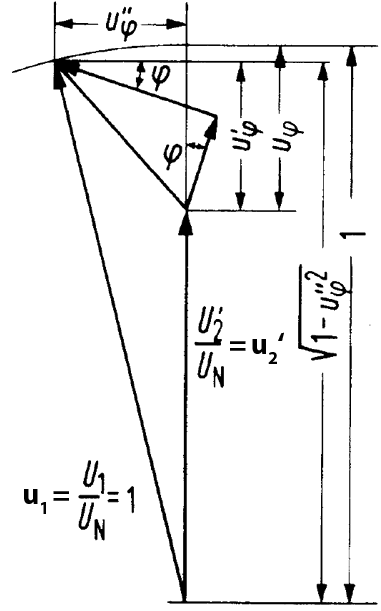
\includegraphics[width=3cm]{bilder/KappschesDreieck.png}
		            \end{minipage}
					\begin{minipage}{7.5cm}
		      			$$u_{\varphi} = u_{\varphi'} + 1 - \sqrt{1 - u_{\varphi''}^2}$$
		      			$$ \boxed{u_\varphi \approx u_{\varphi'}}\quad (\text{für }u_z
		      			=\frac{U_Z}{U_{N}} \cdot 100\% < 4 \%)$$
		      			$$u_{\varphi'} = n \cdot u_r \cdot \cos \varphi + n \cdot u_x
		      			\cdot \sin \varphi$$ $$u_{\varphi''} = n \cdot u_x \cdot \cos \varphi - n \cdot u_r \cdot \sin \varphi$$
		      			$$\text{Lastfaktor } n = \frac{I_1}{I_{1N}}$$
		      			$$ u_r = \frac{R_k \cdot I}{U_N} \qquad u_x = \frac{X_k \cdot I}{U_N} $$
		      			$$ U_2 = \frac{U_1}{"u} - \Delta U_2 = \frac{U_1}{"u} - \frac{1}{"u}
		      			U_N u_\varphi $$
		      			$$ \Delta U_2 \approx \frac{1}{"u} \cdot (U_R \cdot \cos \varphi + U_X \cdot \sin \varphi)$$\\
		      		\end{minipage}         
                \end{minipage}\\
				\begin{minipage}{8cm}
					\vspace*{-2cm}
 					\begin{tabular}[c]{p{2.66cm}p{2.66cm}p{2.66cm}}
                     	$\quad \varphi = 0$ & $\quad\varphi > 0$ & $\quad\varphi
                     	< 0$\\ rein ohmsche & induktive & kapazitive\\
                     	Last & Last & Last\\
                     	&&\\
                     	Konstruktion: & 1. $\underline{U}_2'$ senkrecht&\\
                     	& 2. $\underline{I}_1$ mit $\varphi$ zu $\underline{U}_2'$\\
                     	& \multicolumn{2}{l}{3. $\underline{U}_R$ in Phase mit $\underline{I}_1$ }\\
                     	& \multicolumn{2}{l}{4. Kappsches Dreieck $\Rightarrow \underline{U}_1$}
                     \end{tabular}               
                \end{minipage}& \hspace{0.2cm}
				\begin{minipage}{10cm}
		      		Beim kappschen Dreieck wird mit ``genormten'' Gr\"ossen (klein $u$) gerechnet: 
		      		$u = \frac{U_{Strang}}{U_{N, Strang}} = \frac{U_X}{U_N} \qquad
		      		\boldsymbol{U_N = U_1} $\\ \\ Das Kappsche Dreieck dreht sich um die
		      		Spitze der Prim\"arspannung. Bei konstantem Strom und variablem $\cos(\varphi)$ beschreibt ${u}_2'$
		      		einen
		      		Kreis um die Prim\"arspannung.\\ Bei \textbf{kapazitiver Last steigt}
		      		die Sekund\"arspannung über den Leerlaufwert an. \\ 
		      		\textbf{Ähnlichkeitssatz:}\\
		      		\"Andert sich $U_2$ oder $U_1$ so ändern sich alle Gr\"ossen masst\"ablich\\
		      		Bsp.: $\boxed{U_{2_{neu}} = U_{2_{alt}} \cdot \frac{U_{1_{neu}}}{U_{1_{alt}}}}$ \\              
                \end{minipage}     
            \end{tabular}

		
		\subsubsection{Wirkungsgrad des Trafos}
			\begin{tabular}{p{4.5cm}p{7cm}p{7.5cm}}
            	Wirkungsgrad &
            		$\eta = 1- \dfrac{P_V}{P_B} = 1-\dfrac{P_{V0} + P_{VK} \cdot
            		(\frac{P_B}{P_N})^2}{P_B} $ &
            	\begin{minipage}{7cm}
                	$P_B$ = Betriebsnennleistung = $P_1$ = $S_1 \cdot \cos \varphi$\\
                	$P_{N}$ = Nennleistung\\
                	$P_{V0}$ = Leerlaufverlustleistung = $P_{{Fe}_N}$\\
                	$P_{VK}$ = Kurzschlussverlustleistung = $P_{{Cu}_N}$             	
                \end{minipage}\\ \\
            	 &
            		$\eta = 1 - \dfrac{a + (\frac{P_B}{P_N})^2}{P_B} P_{VK}$ &
            	\begin{minipage}{7cm}
 					$a = \dfrac{P_{V0}}{P_{VK}}$ = Verlustverh"altnis                	
                \end{minipage}\\ \\            		
            	 &
            		$\eta = 1 - \frac{P_{V0}+P_{VK}}{P_B} $ 
            		& (bei Wirkleistungsvollast) \\ \\
            	Maximaler Wirkungsgrad
            	& $S_{\eta-max} = \sqrt{a} \cdot S_N$ \quad $P_{\eta-max} = \sqrt{a}
            	\cdot P_N$
            	& (Kupferverluste = Eisenverluste)
            \end{tabular}	

	\subsection{Drehstrom-Leistungstransformatoren} 
	Angegebene Leistung bezieht sich immer auf alle drei Wicklungen. $\Rightarrow P_{Wicklung} =
	\frac{P_N}{3}$ \\
	Angegebene Spannungen und Str\"ome gelten immer für Aussenleiter. Somit muss immer entweder - je
 nachdem ob Dreieck- oder Sternschaltung vorliegt -	Strom oder Spannung mit Faktor
 $\frac{1}{\sqrt{3}}$ multipliziert werden.
 	\subsubsection{Bauformen}
	 $$\text{Kennzeichnung} = [a][b][c][d] = \begin{cases}
                  [a] = \text{Oberspannungswicklung, Grossbuchstabe (Y,D,III,Z)
                  }\\
                  [b] = \text{Unterspannungswicklung, Kleinbuchstabe (y,d,iii,z) } \\
                  [c] \cdot 30^\circ = \text{Phasenverschiebung zwischen Unter- und Oberspannung }
                  \\ [d] = 0 \text{, falls Neutralleiter herausgeführt (optional)}
                  \end{cases}$$
		\begin{center}
	    	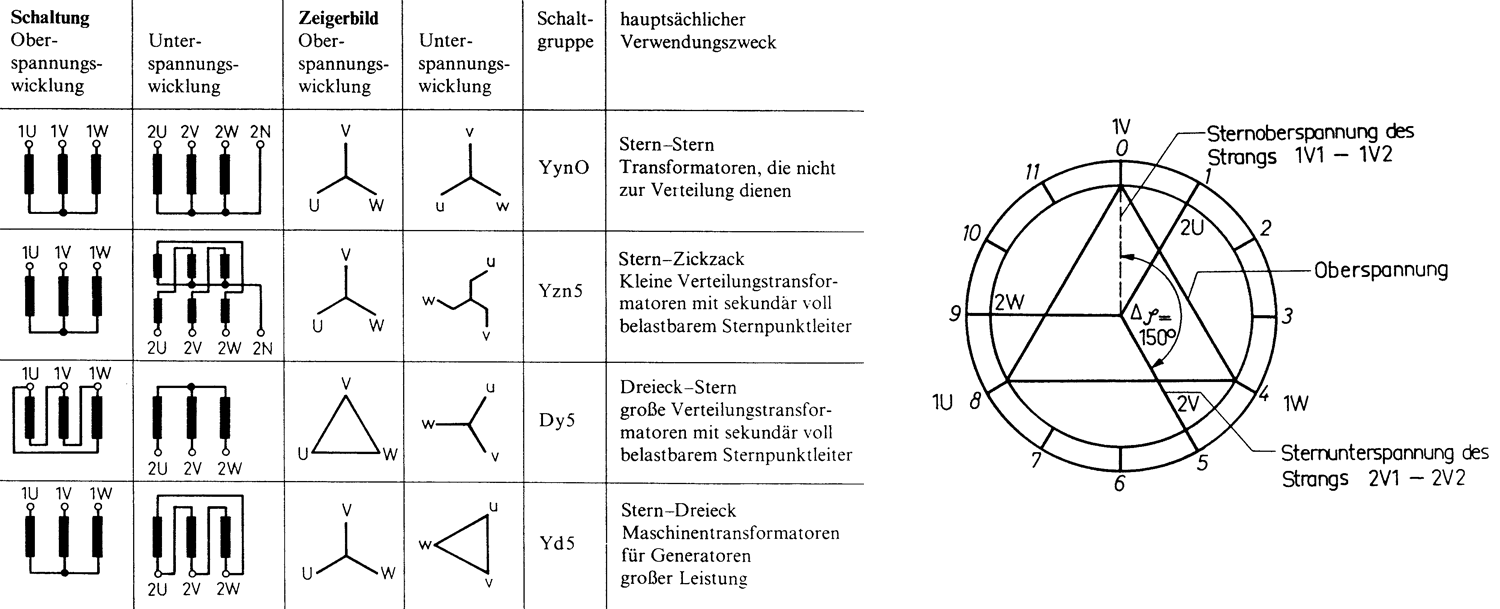
\includegraphics[width=0.99\textwidth]{bilder/Drehstromtrafo.png}
	    \end{center} 
	    
\subsection{Zeigerdiagramme}
\begin{minipage}{0.33\textwidth}
\textbf{Unbelasteter Trafo}\\
\includegraphics[width=0.99\textwidth]{bilder/trafo_leerlauf.png}
\end{minipage}
\begin{minipage}{0.33\textwidth}
\textbf{Belasteter Trafo}\\
\includegraphics[width=0.99\textwidth]{bilder/trafo_nennlast.png}
\end{minipage}
\begin{minipage}{0.33\textwidth}
\textbf{Kurzgeschlossener Trafo}\\
\includegraphics[width=0.99\textwidth]{bilder/trafo_kurz.png}
\end{minipage}
	    
%TODO: Im Parallelbetrieb

	    
